\chapter{Noosfero}
\label{cap:noosfero}
%Introdução
Neste capítulo iremos discutir o funcionamento e arquitetura do software livre Noosfero\footnote{Maiores informações em: \url{http://www.noosfero.org}}, a plataforma de redes sociais.


\section{Noosfero: A Plataforma Utilizada no Participa.br}
%Contexto
O Noosfero é uma plataforma livre para criação de redes sociais, que está disponível sob licença AGPL\footnote{Licença de software GNU Affero General Public License} V3. O Noosfero tem como objetivo permitir a criação de uma rede social por parte de um usuário, onde o mesmo pode modificá-lo e personalizá-lo de acordo com suas necessidades. No entanto, o Noosfero também pode ser adaptado para ser utilizado como um Sistema de Gerenciamento de Conteúdo (CMS), ou até mesmo funcionando em portais de economia solidária.

A Colivre\footnote{Maiores Informações em: \url{http://www.coolivre.coop.br}} (Cooperativa de tecnologias livres) é a criadora/mantenedora do Noosfero, ela é uma cooperativa sediada em Salvador/BA. Essa cooperativa trabalha exclusivamente com softwares livres, dentre eles, manutenção de redes sociais que utilizam o Noosfero, sites em geral, intranets com Wiki, capacitação de usuários, consultorias, entre outros. Atualmente os desenvolvedores da Colivre mantém o repositório do Noosfero, isto é, eles são responsáveis por revisar os códigos que são enviados pela comunidade e integram ao código do Noosfero.

O Noosfero é escrito na linguagem de programação \textit{Ruby} versão 1.9.2 (discutido na seção \ref{sec:linguagemruby} e utiliza framework para aplicações web \textit{Ruby on Rails} versão 3.2 (mais detalhes na seção \ref{sub:frameworkrails}. Utiliza também os padrões arquiteturais de software \textit{Model-View-Controller} (MVC), que será discutido na seção \ref{sub:arquiteturamvc} e o padrão básico de plugins, discutido na seção \ref{sub:arquiteturaplugin}. 

A escolha da linguagem \textit{Ruby} foi decisiva no Noosfero, pois possui uma sintaxe simples, que facilita a manutenibilidade do sistema, característica importante em projetos de software livre que tendem a atrair colaboradores externos a equipe. E o \textit{Rails} como será visto mais adiante na seção \ref{sub:frameworkrails}, possui conceitos que auxiliam em sua produtividade. \cite{meirelles2013metricas}

\section{A Arquitetura de Funcionamento do Noosfero}

Detalhar alguns dos padrões arquiteturais utilizado no Noosfero é importante para um maior entendimento sobre os elementos essenciais de sua arquitetura e como eles se relacionam, ajudando a evoluir o software de maneira correta, deixando de lado detalhes desnecessários e irrelevantes. Sendo assim, entender a arquitetura de funcionamento do Noosfero é um dos passos iniciais para evolução do Participa.br, e consequentemente atingir os objetivos desta monografia.

A arquitetura de software é definida pela estrutura ou estruturas utilizadas pelo sistema, que são os componentes que fazem parte do software, assim como suas relações, além das propriedades que são visíveis externamente e as relações desses componentes \cite{bass1998architecture}. Já para Garlan (\citeyear{garlan1995architecture}) se resume como a estrutura de todos componentes  daquele software, assim como suas relações e especificações que vão desde a concepção, desenvolvimento e evolução durante ao longo do ciclo de vida.


Fowler \citeyear{fowler2006padroes} em seu estudo, mostra que a definição do termo arquitetura em relação a software é bastante confusa e contraditória. Vários autores não concordam sobre uma definição especifica e definem de maneira errônea, então podem existir diversas outras definições na internet.

Na figura \ref{fig:arquiteturanoosfero}, é apresentado a arquitetura básica de funcionamento do Noosfero. As próximas seções vão explicar algumas decisões que foram tomadas no desenvolvimento do mesmo.

\graphicspath{{figuras/}}
\begin{figure}[h]
\centering
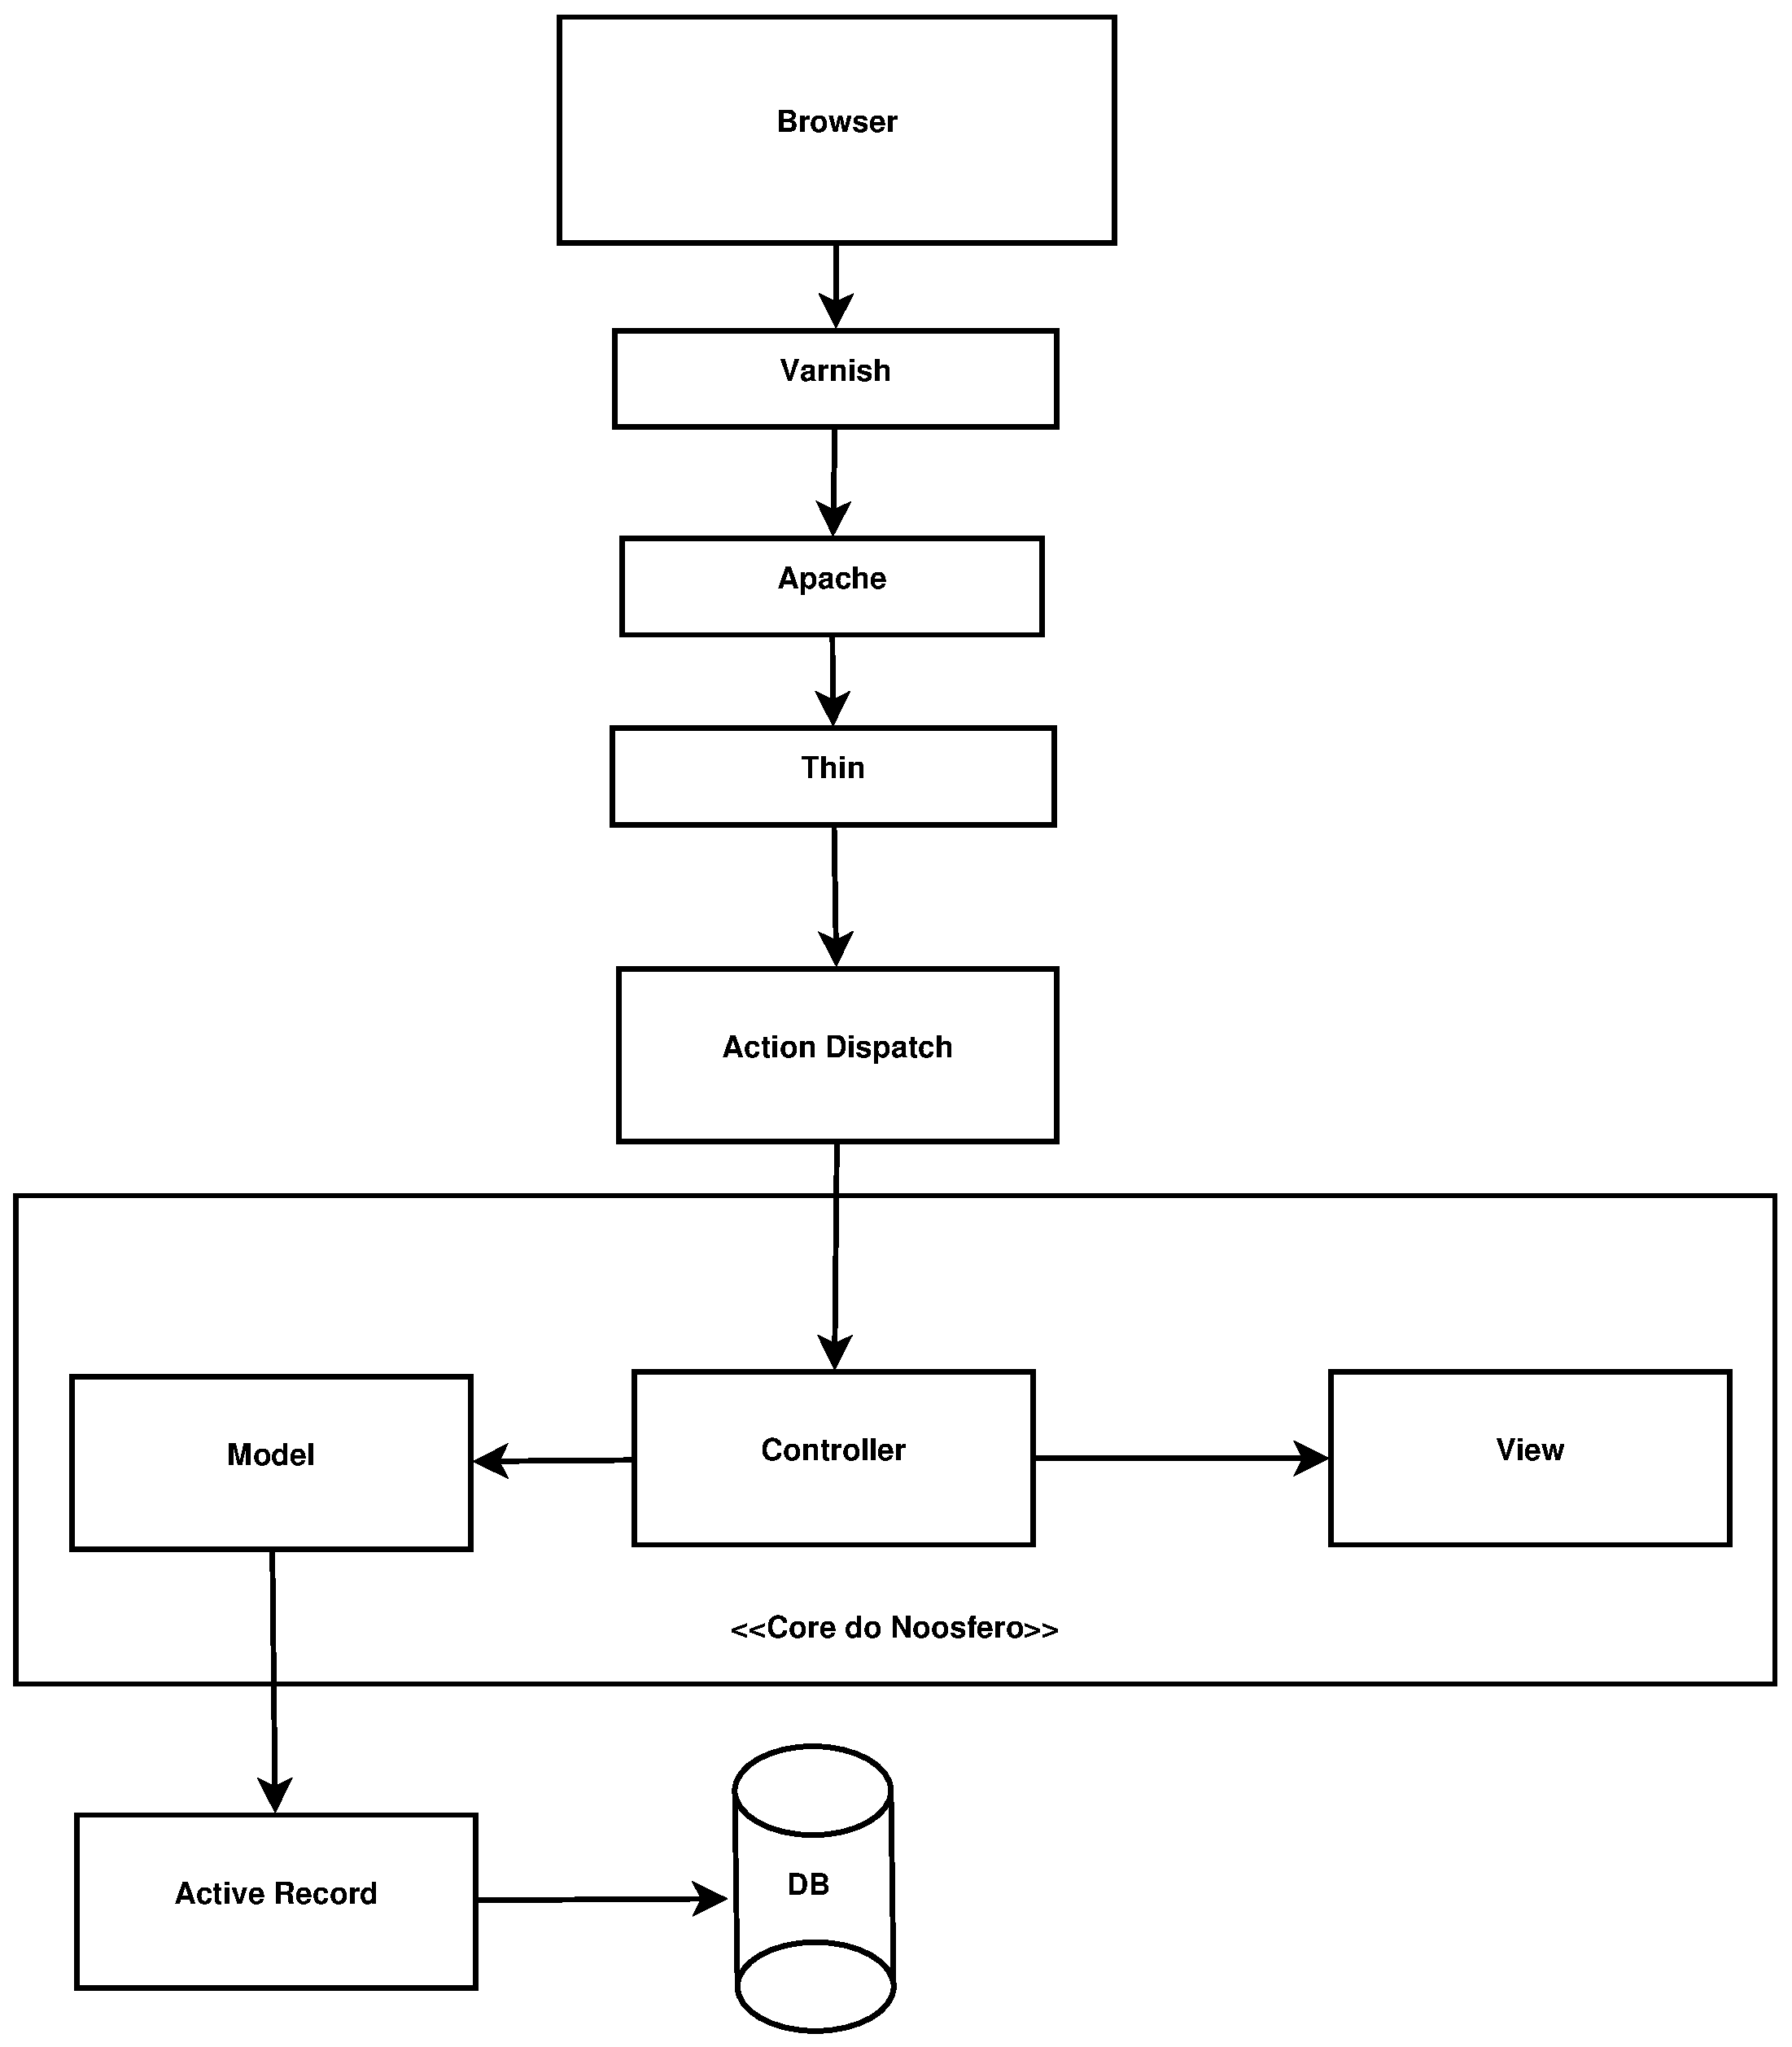
\includegraphics[width=0.9\textwidth]{noosfero_architeture}
\caption[Arquitetura de funcionamento do Noosfero]{Arquitetura de funcionamento do Noosfero. Extraído de \cite{bucher2013rede}}
\label{fig:arquiteturanoosfero}
\end{figure}

\subsection{A Linguagem de Programação \textit{Ruby}}
\label{sec:linguagemruby}

O Ruby é uma linguagem de script, que possui similaridades com o Perl e outras linguagens de script. Ruby possui uma programação interpretada~\footnote{Linguagem executada através de um interpretador} multiparadigma~\footnote{Linguagem que possui mais de um paradigma} de tipagem dinâmica~\footnote{Não exige a declaração do tipo da variável, que pode mudar durante a execução do programa} ou forte~\footnote{É possível declarar o tipo da variável (inteiros, caractere, entre outros)}, desenvolvida no Japão em 1995 por Yukihiro ``Matz‘‘ Matsumoto. O criador da linguagem ``Matz‘‘, diz que a linguagem Ruby, tem como um dos principais pontos ser ``simples, direto ao ponto, extensível e portável‘‘, além de ser totalmente livre.

Uma das vantagens da linguagem \textit{Ruby} é o fato dela ser multiplataforma, isto é, ela é capaz de rodar em diversos sistemas operacionais como Windows, Linux e Mac OS.

Outra vantagem da linguagem \textit{Ruby} é o fato dela possuir gemas (\textit{gems}), que são bibliotecas externas que podem ser reaproveitadas pelos usuários. Essas bibliotecas são fornecidas através de um repositório chamado de \textit{RubyGems}\footnote{Informações em: \url{https://rubygems.org/}}, ou seja, caso o desenvolvedor necessite realizar uma autenticação para o seu sistema, ele pode reaproveitar alguma gema que cuide da autenticação, diminuindo o reuso de código e aumentando a produtividade.

\subsection{Extendendo o \textit{Ruby} para Aplicações Web Através do \textit{Framework Rails}}
\label{sub:frameworkrails}

O \textit{Rails} é um arcabouço de desenvolvimento web escrito na linguagem \textit{Ruby}, ele foi disponibilizado no ano de 2004 por David Heinemeier Hansson. O \textit{Rails} possui como uma das suas principais premissas facilitar o desenvolvimento de aplicativos, pois sua concepção e arquitetura permitem ao programador uma produtividade maior, isto é, com o \textit{Rails} é possível criar uma aplicação completa com conexão com banco de dados em pouco tempo. 

O \textit{Ruby on Rails} foi utilizado nas primeiras versões do \textit{Twitter}~\footnote{O Twitter em suas primeiras versões usava o \textit{Ruby on Rails}, no entanto por baixo desempenho migrou para Java. Maiores Informações em:\url{http://engineering.twitter.com/2011/04/twitter-search-is-now-3x-faster_1656.html} \label{ft:twitterjava}}, GitHub \footnote{Disponível em: \url{http://www.github.com}} e Scribd \footnote{Disponível em: \url{http://www.scribd.com}}. O \textit{Rails} utiliza vários princípios em sua arquitetura para orientar desenvolvimento do ``modo certo‘‘ ou ``Rails way‘‘, possibilitando o programador focar o seu desenvolvimento no problema do cliente, deixando a parte da estrutura da aplicação por conta do arcabouço. \cite{meneses2014mezuro}

O arcabouço \textit{Ruby on Rails} influencia em maior produtividade graças a conceitos como:

\begin{itemize}
\item DRY - \textit{Don’t Repeat Yourself} - É um conceito que evita a duplicação de código fonte, onde propõe que um mesmo trecho de código deve possuir representação único no sistema. Isso garante que uma alteração no software seja realizada em um único local no código, evitando código duplicado e facilitando a manutenibilidade do sistema.
\item Paradigma de Programação Orientado à Convenção \textit{Convention Over Configuration} - Esse paradigma facilita o desenvolvimento de software, pois diminui o tempo que o programador gasta integrando serviços e configurando todo os seus módulos (banco de dados, ferramentas para teste, entre outros). Nesse paradigma o desenvolvedor pode se preocupar com a lógica de negócio, deixando a lógica de aplicação à cargo do suporte orientado à convenção sobre configuração.
\item REST \textit{(\textbf{RE}presentaional \textbf{S}tate \textbf{T}ransfer.)} É um estilo arquitetural para aplicações web. Ele propõe princípios (não exclusivos ao REST) que definem
como \textit{Web Standards} como HTTP e URIs devem ser usados.
\item Múltiplos ambientes - \textit{No Rails}, cada aplicativo possui três ambientes. Um desses ambientes é voltado para o desenvolvimento do software em si, outro para testar o software através de testes e mais uma utilizada para o software entrar em produção. Cada um desses ambientes possuem comportamentos quase iguais, no entanto, cada um utiliza um banco de dados diferente.
\end{itemize}

Devido ao fato do Noosfero ter sido desenvolvido em cima do arcabouço \textit{Ruby on Rails}, sua arquitetura é altamente ligada a arquitetura do mesmo. Essa arquitetura é ilustrada pela figura \ref{fig:arquiteturaror}.

\graphicspath{{figuras/}}
\begin{figure}[H]
\centering
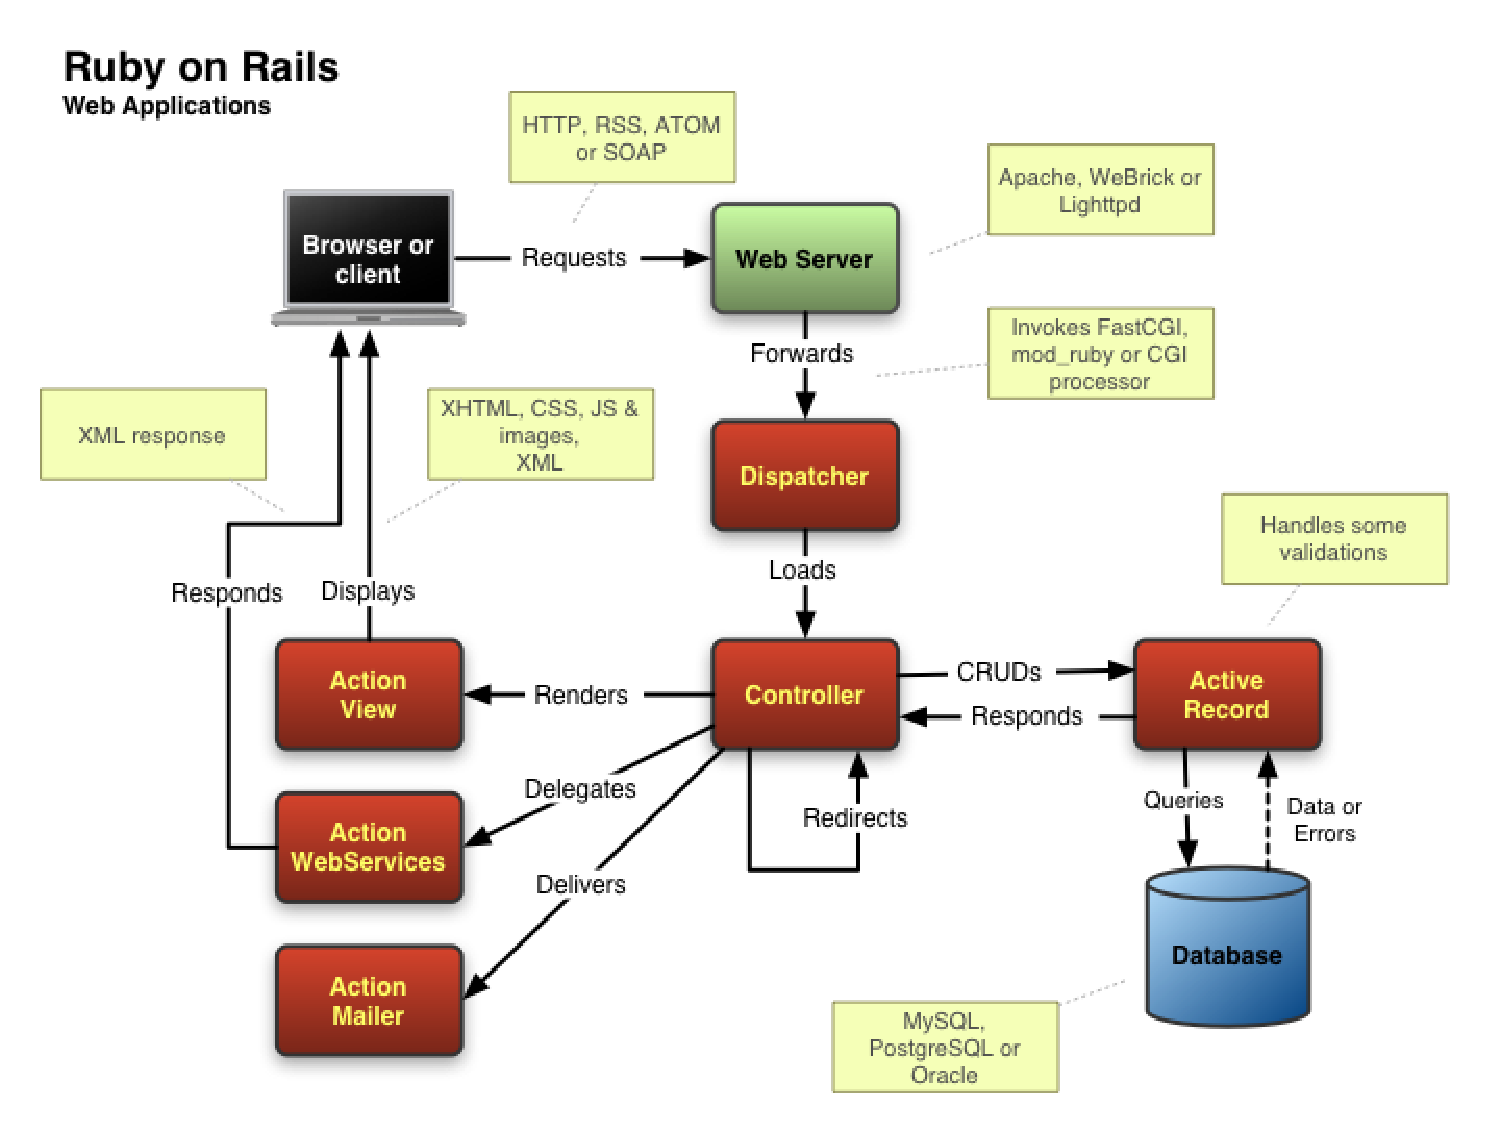
\includegraphics[width=1.1\textwidth]{rails-overview}
\caption[Arquitetura de funcionamento do \textit{Ruby On Rails}]{Arquitetura de funcionamento do \textit{Ruby On Rails}. Extraído de \cite{mejia2011rails}}
\label{fig:arquiteturaror}
\end{figure}

Nessa figura \ref{fig:arquiteturaror}, são observado alguns componentes que fazem parte do \textit{Ruby On Rails}. Esses componentes são.

\begin{itemize}
	\item \textit{Action Pack} - Esse módulo compõe os gerenciadores dos controladores e vistas do \textit{Ruby on Rails}, que serão discutidos no módulo \ref{sub:arquiteturamvc}. Esses dois módulos são responsáveis por receber as requisições do cliente e renderizam a resposta de volta para o cliente. Os três componentes que fazem parte do \textit{Action Pack} são detalhados abaixo:
	\begin{itemize}
		\item \textit{Action Controller} - Responsável por realizar o mapeamento de todas as controladoras (\textit{controllers}) em uma aplicação \textit{Rails}. Ele recebe as requisições que chegam através de um navegador (\textit{browser}), tratando cada ação e enviando para o determinada função.
		\item \textit{Action View} - Quando uma requisição chega, ela é enviada para \textit{Action Controller}, que trata e chama a \textit{Action View} para devolver a resposta da requisição. gerencia as views da aplicação. Isto é, ele renderiza as saídas de volta para o cliente dentro de templates em formato HTML e XML por padrão e inclui suporte embutido para \textit{Javascript, AJAX, jQuery}.
		\item \textit{Action Dispatch} - É responsável por trabalhar tratando o protocolo HTTP, fazendo a obtenção dos cabeçalhos, determinando tipos \textit{MIME}, sessão, cookies e outras atividades.
	\end{itemize}
	\item \textit{Action Mailer} - É responsável por toda a lógica inerente a criação e funcionamento de e-mails, como enviar mensagem de boas vindas, recuperar senha, Envia e-mails baseados em templates criados na Action View, que são renderizados da mesma maneira que uma resposta a uma requisição.
	\item \textit{ActiveRecord} - É um \textit{Object-Relational-Mapping}, ou seja, uma biblioteca que faz o mapeamento de estruturas relacionais que estão no banco de dados para objetos \textit{Ruby} diretamente no paradigma de orientação a objeto.
	\item \textit{Railties } - É responsável pela geração automática do código do Ruby, quando por exemplo, é criada alguma aplicação, ou gerado alguma classe de forma automática (através do \textit{scaffolding}).  
	\item \textit{ActionSupport} -  É uma coleção de classes úteis  utilizados para o desenvolvimento de aplicações \textit{Ruby on Rails}, incluindo suporte para internacionalização, testes, entre outros.
\end{itemize}


\subsection{Arquitetura MVC}
\label{sub:arquiteturamvc}

O padrão arquitetural MVC (\textit{\textbf{M}odel \textbf{V}iew \textbf{C}ontroller})foi desenvolvido por Trygve Reenskaug nos anos 70. Segundo Fowler (\citeyear{fowler2006padroes}), o MVC tem exercido grande influência nos projetos de interface com o usuário, isso inclui o \textit{Ruby On Rails}.

O arcabouço para aplicações web \textit{Ruby On Rails} apoia a utilização  MVC, que sugere que o software deve ser dividido em componentes, separando em camadas de persistência, logica e interface. Isso torna o desenvolvimento do software muito mais organizado, claro e enxuto, facilitando a manutenção e evolução do sistema e com mantém a segurança do software em fases posteriores do seu desenvolvimento \cite{silva2012mvc}. Porém, o baixo acoplamento e alta coesão de um software, com módulos responsáveis só é garantido se houver uma organização do sistema em camadas, garantindo assim a escalabilidade, eficiência e a reusabilidade. Na figura \ref{fig:figuramvc}, temos a arquitetura de funcionamento da arquitetura MVC.

\graphicspath{{figuras/}}
\begin{figure}[H]
\centering
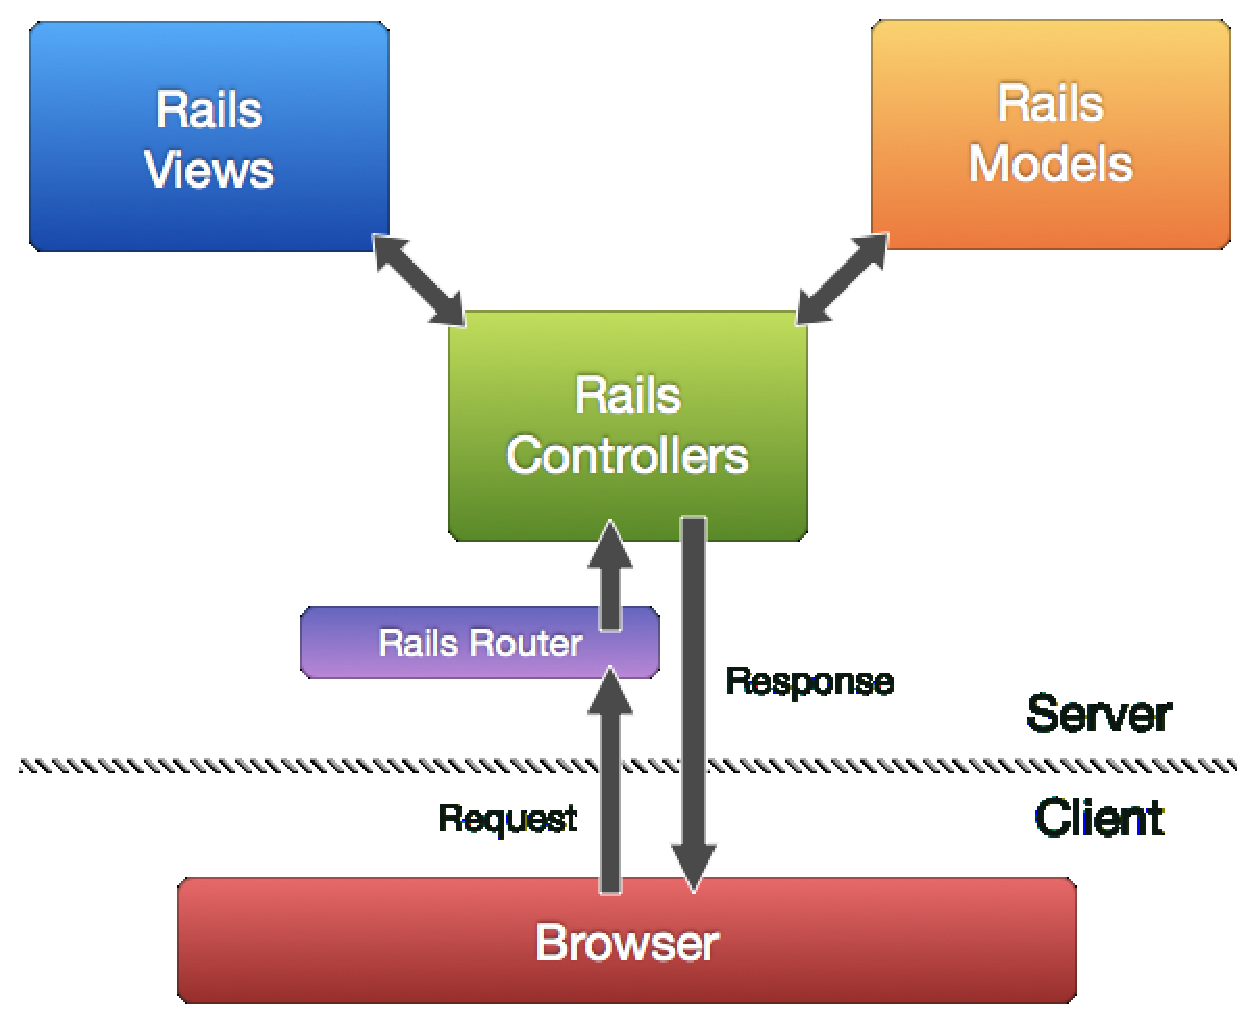
\includegraphics[width=0.9\textwidth]{funcionamentomvc}
\caption[Funcionamento do \textit{Model View Controller}]{Funcionamento do \textit{Model View Controller}. Extraído de \cite{monim2013mvc}}
\label{fig:figuramvc}
\end{figure}

Nessa visão em camadas, (i) o modelo (\textit{model}) possui informações sobre a regra de negócio, comportamentos e dados que não são utilizados na interface de usuário, (ii) a vista (\textit{view}) é composta pela saída que é vista pelo usuário do sistema, por exemplo, uma página HTML, (iii) o controlador (\textit{controller}) é responsável por receber as requisições (entradas) enviadas pelo cliente e decide qual o modelo que deve ser utilizado por aquela requisição e faz com que a vista seja renderizada para o usuário como reposta da requisição. Essa combinação entre vista e controladora é chamada de interface de usuário \cite{fowler2006padroes}. Já o (iv) roteador possui um mapeamento de todas as URLs das requisições, essas URLs são enviadas diretamente para a controladora responsável.

No Noosfero a implementação do padrão arquitetural MVC é obedecida, pois o mesmo é inerentes ao arcabouço utilizado.

\subsection{Plugins: Uma Arquitetura Extensível no Noosfero}
\label{sub:arquiteturaplugin}
%Arquitetura de plugins do Noosfero
O Noosfero também utiliza uma arquitetura extensível através do uso de plugins. Essa arquitetura é interessante, pois como dito anteriormente, o Noosfero implementa a arquitetura de múltiplos ambientes presente no arcabouço \textit{Ruby On Rails}. Cada um desses ambientes possuem comportamentos que requerem implementações diferentes.
 
Essa arquitetura encoraja a criação de um software modular, ou seja, a criação de módulos específicos para cada função diminuindo o acoplamento, aumentando a coesão e definindo bem as responsabilidades de cada módulo \cite{rozanski2005architecture}.  

Uma das grandes vantagens em se criar uma aplicação com arquitetura extensível através de plugins, é o fato de o desenvolvedor criarem novas funcionalidades sem ter acesso ao código fonte do software, apenas é necessário somente a API~\footnote{Acrônimo \textbf{A}pplication \textbf{P}rogramming \textbf{I}nterface, que são padrões definidos por um software para utilização de seus recursos sem a necessidade de entrar na implementação do código fonte do software} que é fornecida pelo fabricante do software. Apesar disso no Noosfero os plugins são mantidos na linguagem \textit{Ruby}, através do arcabouço \textit{Ruby on Rails} e acoplados juntamente com o código principal (núcleo), dentro de uma pasta “plugins”, isso ajuda no controle de qualidade do código. Quando houver a necessidade de alterar o código do Noosfero, os testes dos plugins são executados para verificar se as mudanças não afetaram seu funcionamento~\footnote{Maiores informações em: \url{http://noosfero.org/Development/Plugins}}.

O funcionamento dos plugins é inspirado no paradigma de orientação a eventos, onde núcleo do Noosfero dispara um evento durante a execução de alguma função, e os plugins interessados nesse evento vão sobrescrever o método do core do Noosfero tratando o evento de acordo com sua implementação, funcionando como o padrão de projeto \textit{Composite}. Os eventos que são chamados pelo pelo Noosfero e implementados em outras partes são chamados de “hotspots”.

\subsection{Arquitetura Lógica do Noosfero}

Uma das desvantagens do arcabouço Ruby on Rails está em lidar com grande números de usuários, um dos motivos é o péssimo suporte para aplicações \textit{multithread}~\footnote{Softwares que utilizam vários núcleos para processamento}, como foi visto no caso de estudo do Twitter~\footref{ft:twitterjava}. O Noosfero utiliza uma arquitetura lógica que tenta minimizar o processamento gasto com o carregamento de imagens, páginas, entre outros, através do sistema de Cache inteligente. Outra solução é a utilização de vários núcleos em seu servidor de aplicação, melhorando o tempo de requisição.

Outro fator importante a ser ressaltado é que o Noosfero utiliza os pacotes homologados pelos desenvolvedores do Debian na versão \textit{stable} (estável). Essa medida trás impactos positivos em relação a segurança do software, já que as correções de vulnerabilidades são feitas diretamente nos pacotes disponibilizados pelos desenvolvedores do sistema operacional, que geralmente são mais rápidos. Abaixo são listados alguns componentes da arquitetura lógica do Noosfero.

\subsubsection*{Varnish}

Varnish~\footnote{Maiores informações em: \url{https://www.varnish-cache.org/about}} é um proxy HTTP reverso que armazena o conteúdo (páginas, scripts, folha de scripts e imagens) requisitado no servidor, evitando múltiplas requisições desnecessárias e consequentemente fazendo com que o servidor deixe de consultar e processar o mesmo conteúdo diversas vezes.

Em uma instalação padrão o Varnish não é configurado, mas é aconselhado que os servidores utilizados em modo de produção configurem e utilizem o Varnish por causa da melhoria de performance obtida com sua utilzação.

\subsubsection*{Apache}

O Apache é um servidor web. Sua função na arquitetura do Noosfero é utilizado como servidor de proxy reverso, isto é, ele fica responsável por encaminhar as requisições recebidas para a porta 80 para uma das instâncias do Thin (que por padrão escutam na porta 50000).

\subsubsection*{Thin}

O Thin é um servidor de aplicações que fica escutando (\textit{listening}) em uma determinada porta (por padrão 50000). Após a chegada de uma requisição vinda de um cliente, uma instância do thin que está disponível se encarrega de encaminhá-la para o Noosfero que se encarrega de processá-la. O Thin suporta que duas instâncias de escuta sejam colocadas a cada núcleo de processamento do sistema hospedeiro, isso aumenta a performance e diminui o tempo de resposta da aplicação.

\subsubsection*{Memcached}

O Memcached~\footnote{Informações em: \url{http://memcached.org/}} é um sistema de cache em memória utilizado para melhorar a performance dos sites dinâmicos, cacheando objetos na memória do servidor, diminuindo a quantidade de acessos ao banco de dados.

\subsubsection*{PostgreSQL}

O PostgreSQL\footnote{Disponível em: \url{http://www.postgresql.org/about/}} é um sistema de gerenciamento de banco de dados relacional de objetos desenvolvido como software livre. O Noosfero é homologado para uso com o banco de dados PostgreSQL.

\section{Entendendo o Domínio de Funcionamento do Noosfero}
\label{sub:dominionoosfero}

Nessa seção será apresentada o modelo de domínio do Noosfero, essencial para o entendimento do sistema e consequentemente para a evolução do mesmo.

Como o Noosfero foi desenvolvido em 2007, o esquema de funcionamento de classes possui uma pequena influência da rede social que havia mais usuários na época, o Orkut\footnote{Disponível em: \url{http://www.orkut.com.br}}. Podemos citar como exemplo dessa influência, a aparência e disposição a disposição de alguns botões, o esquema de comunidade, funcionamento de perfis, entre outros. Na figura \ref{fig:relperfisambientes}, é explicado o funcionamento geral do Noosfero.

\graphicspath{{figuras/}}
\begin{figure}[H]
	\centering
	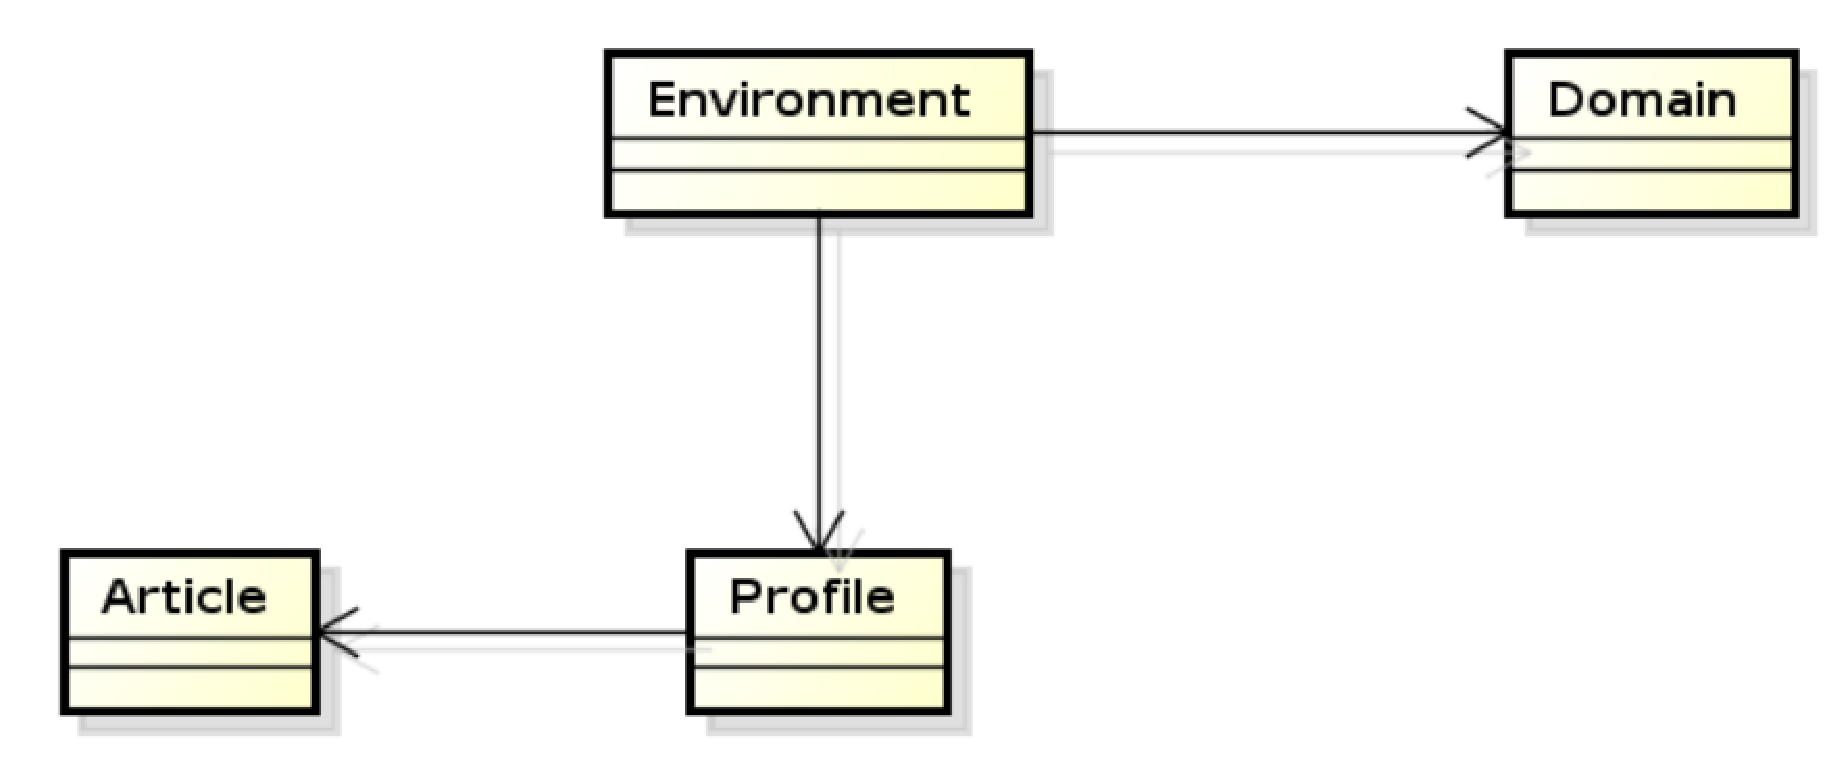
\includegraphics[width=0.8\textwidth]{dominio-ambiente}
	\caption[Relacionamentos entre perfis, ambientes e domínios]{Relacionamentos entre perfis, ambientes e domínios. Extraído de \cite{bucher2013rede}}
	\label{fig:relperfisambientes}
\end{figure}

Como visto na seção~\ref{sub:arquiteturamvc}, o Ruby on Rails possui suporte para múltiplos ambientes dentro de uma única instalação, ou seja, é possível ter um ou mais ambientes de rede social utilizando uma única instalação do Noosfero, basta que o ambiente criado tenha um domínio (\textit{Domain}) diferente do primeiro ambiente. No Noosfero, existe uma entidade chamada Perfil (Profile), essa entidade é uma abstração de outras três outras entidades: Pessoas (\textit{Person}), Comunidade (\textit{Community}) e Empreendimento (\textit{Enterprise}), como é visto na figura \ref{fig:reltipoperfil}. A abstração consiste isolar elementos em comum dentro de uma classe pai, enquanto as especialidades são responsabilidade das classes filhas.

\graphicspath{{figuras/}}
\begin{figure}[H]
	\centering
	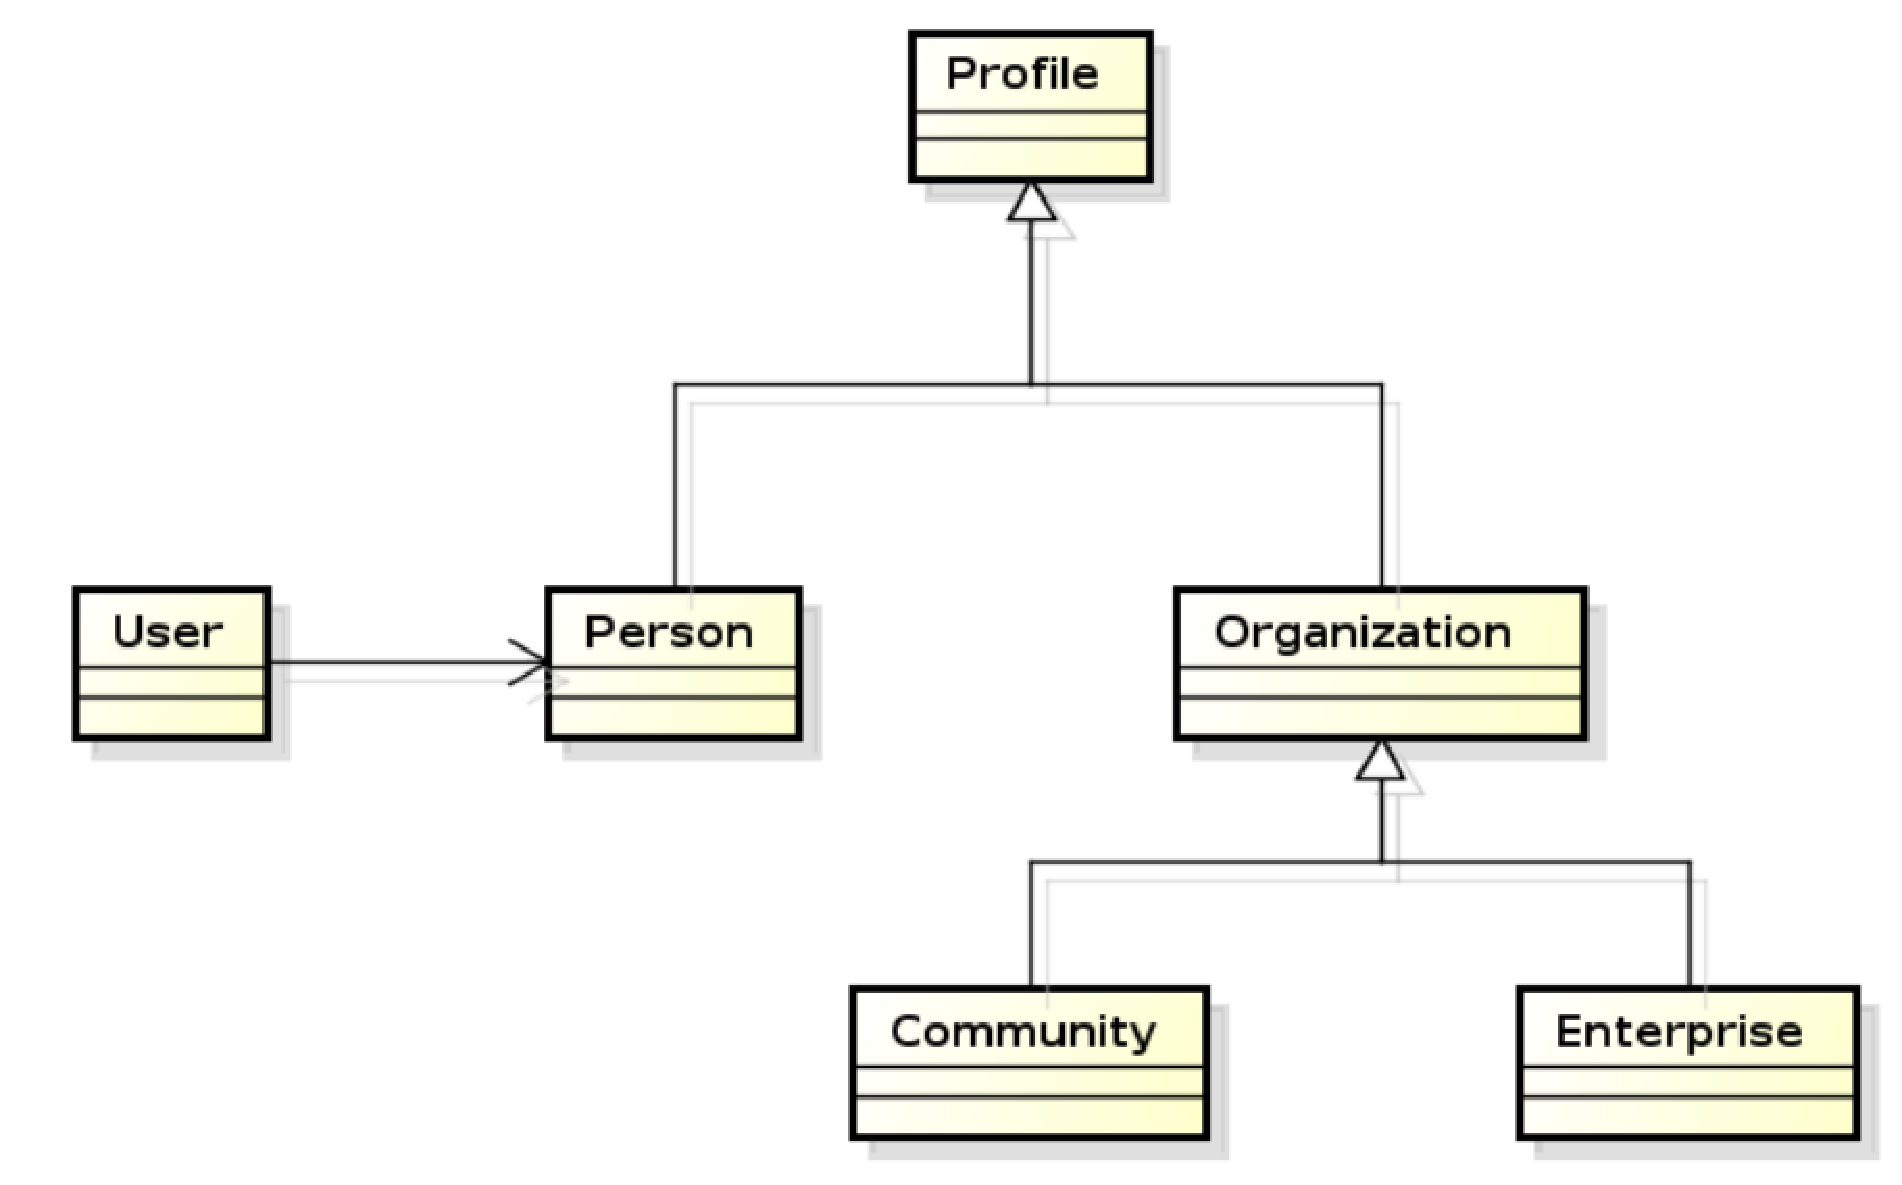
\includegraphics[width=0.8\textwidth]{dominio-profile}
	\caption[Relacionamento entre os tipos de perfis]{Relacionamento entre os tipos de perfis. Extraído de \cite{bucher2013rede}}
	\label{fig:reltipoperfil}
\end{figure}

\graphicspath{{figuras/}}
\begin{figure}[H]
	\centering
	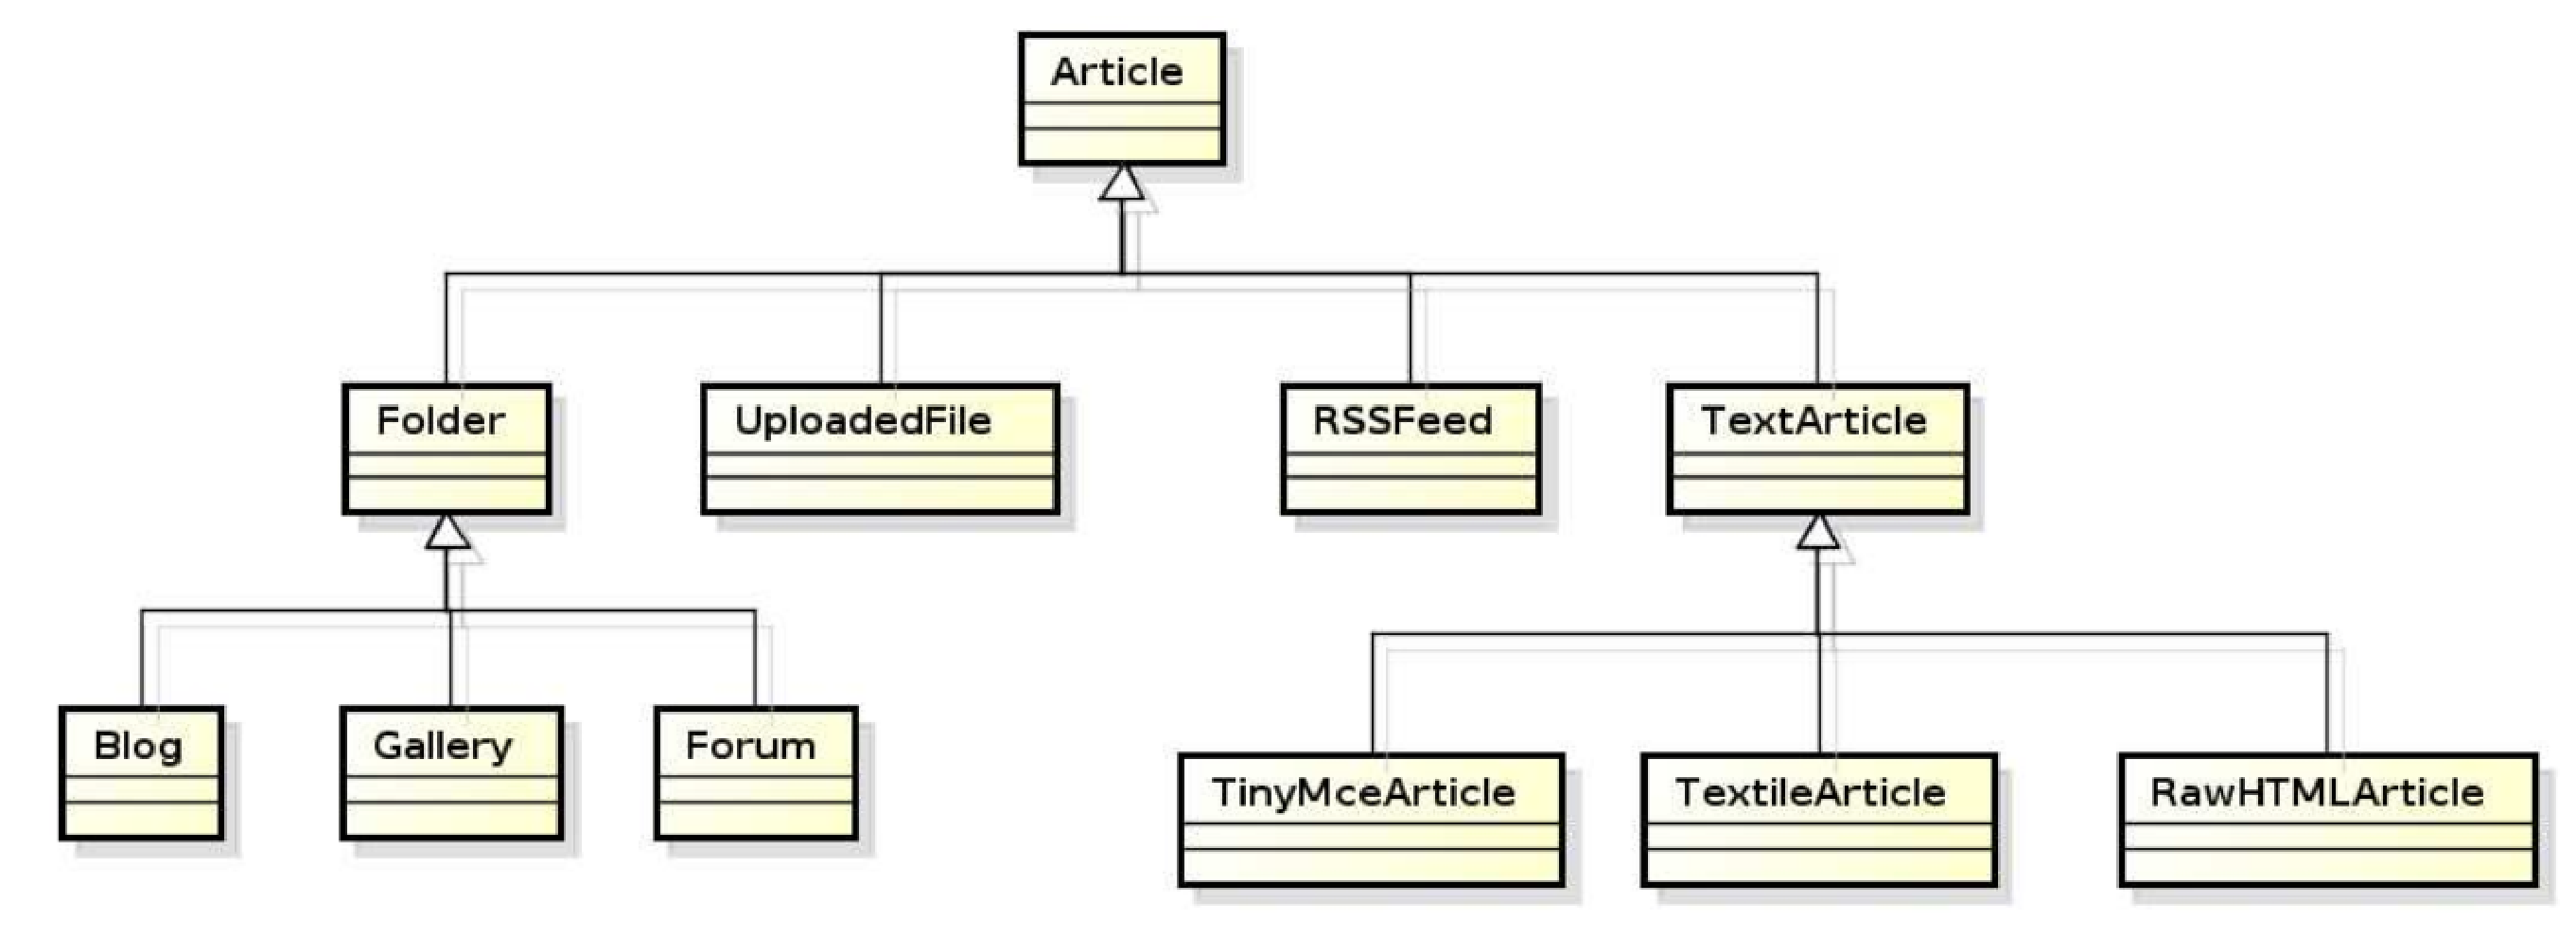
\includegraphics[width=0.9\textwidth]{dominio-artigo}
	\caption[Relacionamento entre os tipos de conteúdo do Noosfero]{Relacionamento entre os tipos de conteúdo do Noosfero. Extraído de \cite{bucher2013rede}}
	\label{fig:tipoconteudo}
\end{figure}

Ainda na figura \ref{fig:reltipoperfil} é encontrada outra abstração no código do Noosfero acontece na classe chamada de organização, que possui o comportamento comum entre comunidades (\textit{community}) e (\textit{enterprise}), visto na figura. A classe usuário (\textit{user}) possui todas as lógicas e implementações relativas a autenticação do usuários, enquanto a classe Person possui lógicas relacionadas a rede social (amigos, manutenção de perfil, etc.), tornando o código mais fácil de ser entendido. Na figura \ref{fig:tipoconteudo} é representado os tipos de conteúdo disponíveis no Noosfero como artigos de texto, fóruns, pastas, artigo usando HTML, blogs de conteúdo, galerias de imagens, arquivos em geral e feeds de notícias. É importante ressaltar que alguns conteúdos que foram implementados no Participa.br, como é o caso do Hub ou trilhas de participação fazem parte de plugins especificos, que estendem os tipos de conteúdo disponíveis.

\section{Desenvolvendo para o Noosfero}

Qualquer pessoa pode ajudar o desenvolvimento do Noosfero/Participa.br, pois como foi visto na seção~\ref{sub:softwarelivre} se trata de um Software Livre. O Noosfero disponibiliza uma lista de novas funcionalidades e bugs a serem corrigidos (\textit{Issue Tracker})~\footnote{Informações em: \url{http://noosfero.org/Development/FeatureItem}}, o qual ajuda novos desenvolvedores sobre quais funcionalidades devem ser desenvolvidas. Essa lista é ilustrado pela figura \ref{fig:issuetracker}.

A Coolivre assim como a comunidade do \textit{Rails}, recomendam que o desenvolvimento do código utilize a técnica de TDD~\footnote{Test Driven Development. Disponível em: \url{http://pt.wikipedia.org/wiki/Test_Driven_Development}}, já que trás um código mais simples, melhor entendível e inspira confiança \cite{beck2003tdd}.

\graphicspath{{figuras/}}
\begin{figure}[h]
\centering
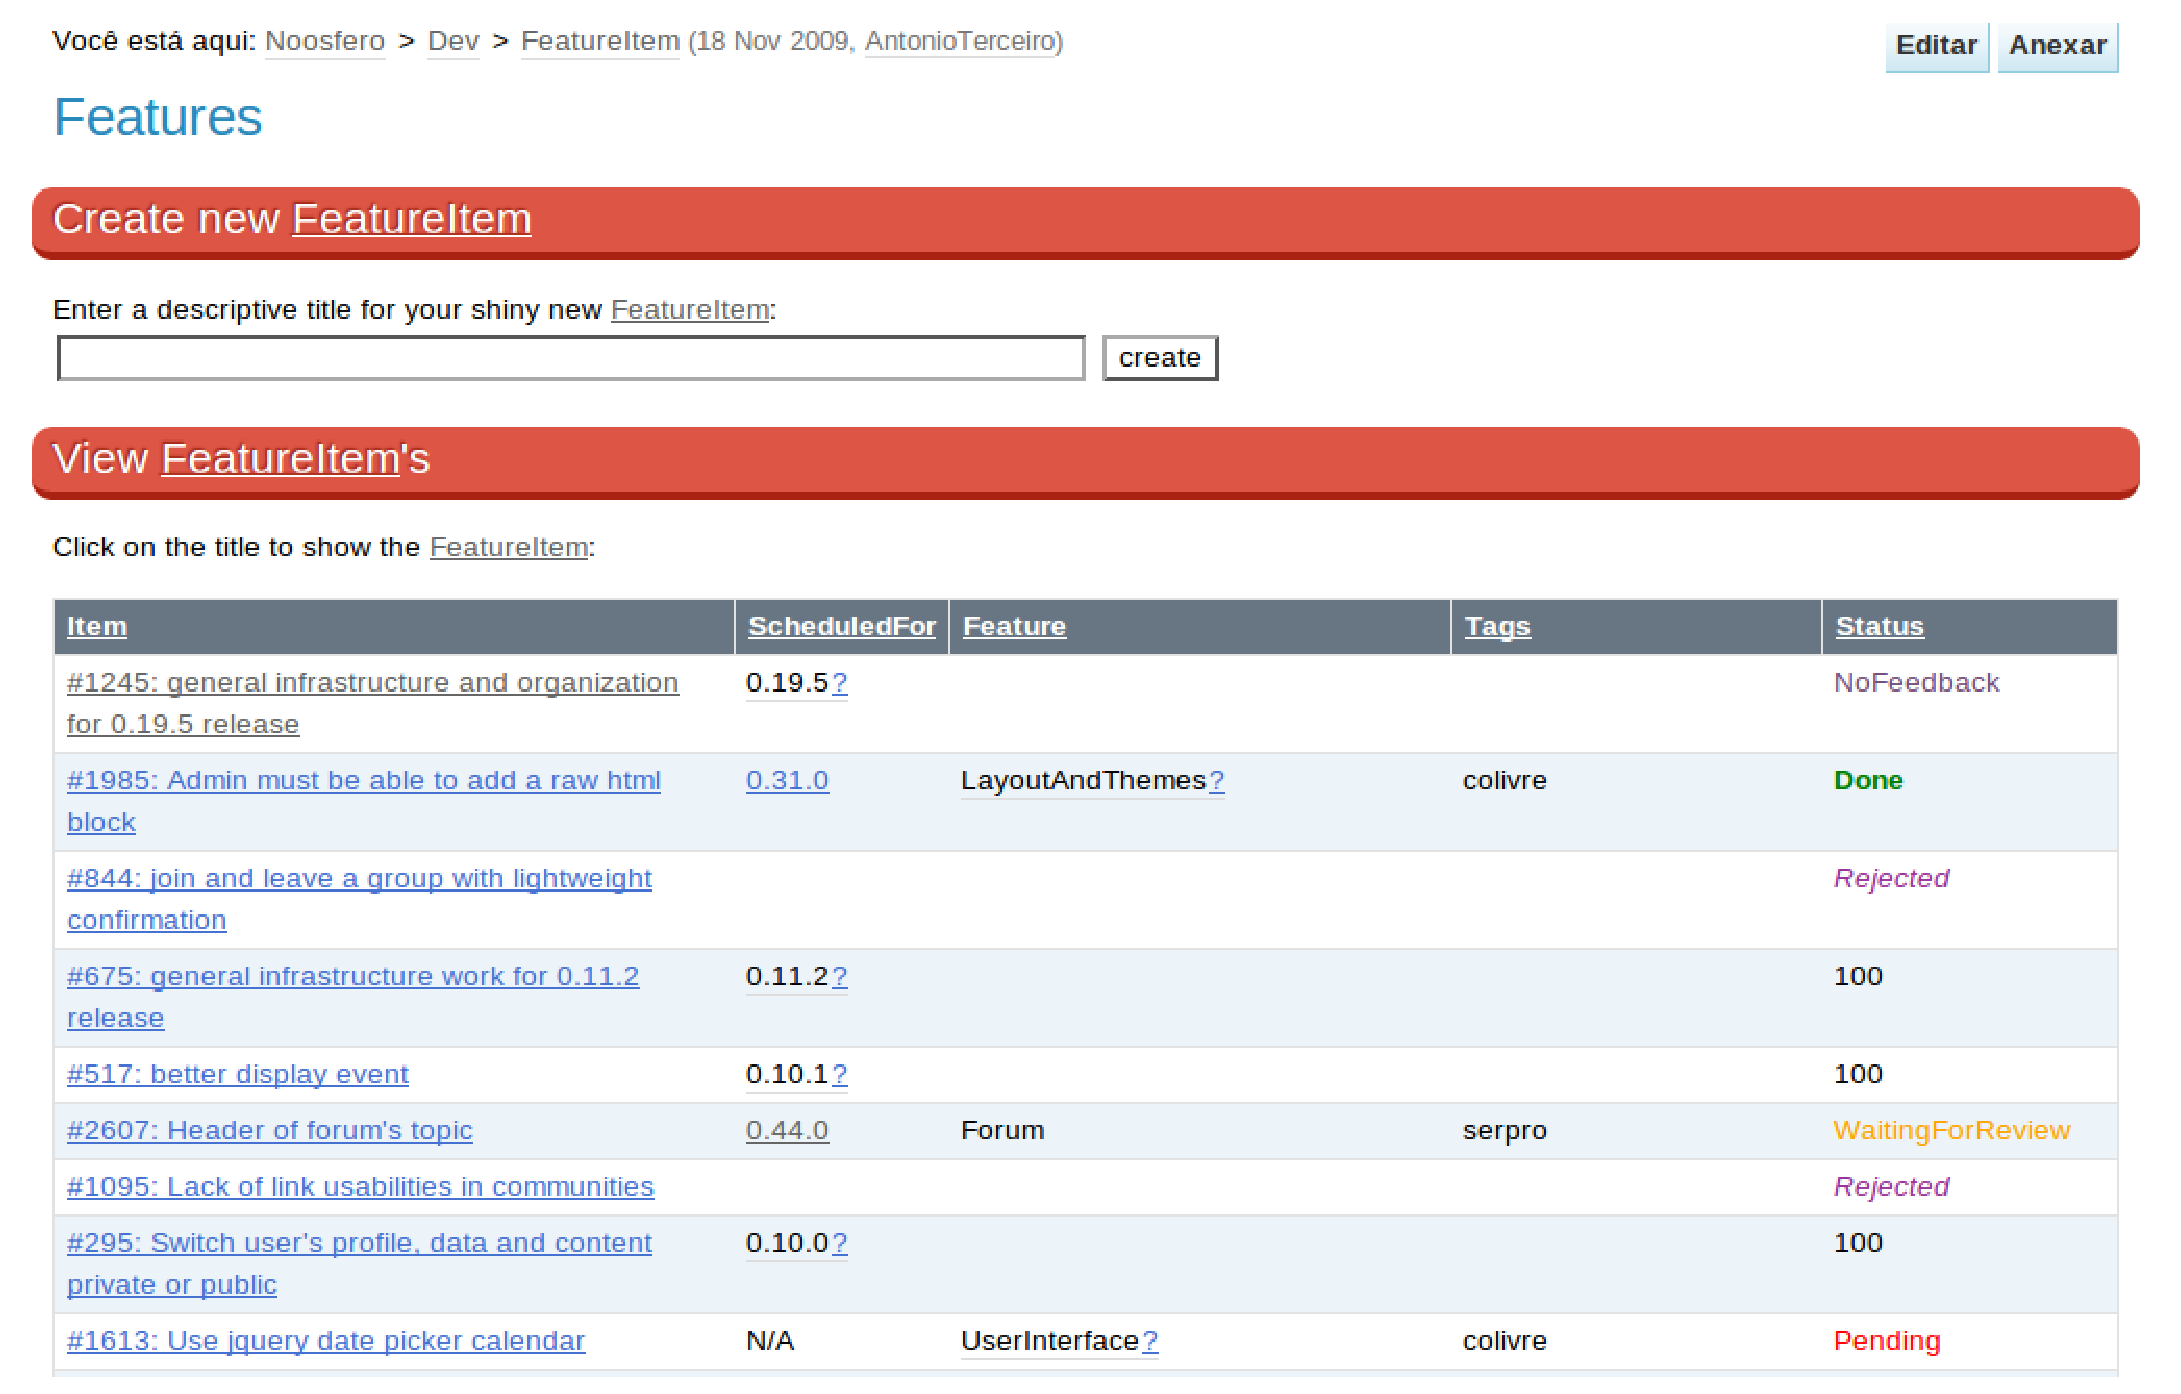
\includegraphics[width=1.0\textwidth]{issue-tracker}
\caption{\textit{Issue tracker} do Noosfero.}
\label{fig:issuetracker}
\end{figure}

Após o desenvolvimento da funcionalidade para o código ser incorporado no Noosfero é necessário que o mesmo seja totalmente testado, fato esse garante que a qualidade do código se mantenha a mesma. O Noosfero utiliza testes unitários~\textbf{Teste responsável por testar pequenas porções do software desenvolvidas em busca da garantia que o todo está funcionando} e testes funcionais~\footnote{Testa se o comportamento do software de acordo com os requisitos planejados, colocando entradas aleatórias e esperando saídas planejadas de acordo com o software} utilizando as ferramentas fornecidas pelo arcabouço \textit{Ruby on Rails}, discutido na seção~\ref{sub:frameworkrails}. Também há testes de aceitação utilizando BDD~\footnote{Behavior Driven Development. Disponível em: \url{http://pt.wikipedia.org/wiki/Behavior_Driven_Development}} através da ferramenta cumcuber, que permite a escrita de testes em linguagem natural.





